
\section{ERD/Class Diagram}

All interactions with the relational database are done via the Django ORM. Furthermore, because the exact data type in the database is dependent upon which database is used (which, currently, is PostgreSQL) the Django ORM data type is listed instead.

Also, because Django converts the Python \texttt{None} value to an empty string before saving it into \texttt{CharField} and \texttt{TextField}s, these fields are marked as nullable although they are not nullable at the database level.

\begin{figure}[h!]
    \centering
    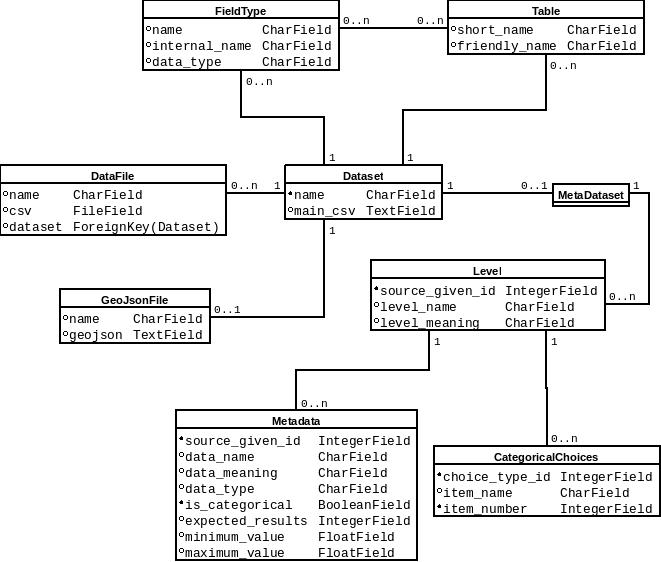
\includegraphics[width=120mm]{images/erd.jpg}
    \caption{The entity relationship diagram (ERD) for ComStat's ORM classes}
    \label{fig:img-comstat-erd}
\end{figure}
